\section{Computation-Risk Tradeoffs for Dropout and Subsampling}
\label{sec:subsampling}

We begin by considering one of the simplest settings, where
the task is to fit a linear regression model according to the least squares
criterion
\begin{equation}
\hat \beta_n = \argmin_\beta \|\Y - \X\beta\|_2
\end{equation}
where $\Y$ is an $n$-vector of response variables, and $\X$ is an
$n\times p$ design matrix of predictor variables, formed from data
$(X_i, Y_i)$, with $X_i\in\reals^p$ and $Y_i\in\reals$, for
$i=1,\ldots, n$, with $n\gg p$.  The computation required
to directly compute the least squares
estimator $\hat\beta_n = (\X^T \X)^{-1} \X^T \Y$ scales as
$O(np^2 + p^3)$.  The first term, $O(np^2)$, is the computation
required to compute the sample covariance $\frac{1}{n} \X^T \X$.
The second term, $O(p^3)$, is the computation required to compute its
inverse, and solve the linear system.
Assuming that the data are generated according to a linear model
$Y_i = X_i^T \beta^* + \epsilon_i$, with $\Var(\epsilon_i) =
\sigma^2$, standard analysis shows the squared error decays as
$\E(\|\hat\beta_n - \beta^*\|_2^2) = O(p/n)$.

A simple way of making a computation-risk tradeoff is to 
subsample the data.  Suppose that $\X_m$ is a random sample
of $m$ rows of $\X$, with corresponding response $Y_m$.
Then the least squares estimator $\hat \beta_m =
(\X_m^T \X_m)^{-1} \X_m^T \Y_m$ 
has error scaling as $\|\hat\beta_m - \beta^*\|_2^2 = O(p/m)$
and computation scaling as $O(m p^2 + p^3)$.  

Subsampling removes entire rows of the data matrix.  As an alternative, suppose that we dropout random entries from $\X$.
In particular, let 
\begin{equation}
\Xdrop = \X \hadamard \bZ
\end{equation}
where $\bZ \sim \text{Bernoulli}(\theta)$ is an $n\times p$ matrix of
$\{0,1\}$ values $Z_{ij} \sim \text{Bernoulli}(\theta_j)$, and 
$\mbf{A}\hadamard \mbf{B}$ denotes the Hadamard (pointwise) product
of matrices $\mbf{A}$ and $\mbf{B}$.  We then compute the
estimator
\begin{equation}
\drop{\beta}_n = \argmin_\beta \|Y - \drop{\X} \beta\|_2 ^2.
\end{equation}

Using fast subspace embedding algorithms, the estimator
$\drop{\beta}_n$ can be computed in time
that scales according to the number of nonzeros in the sparsified
matrix, denoted $\textit{nnz}(\drop{\X})$.   Ignoring approximation error, the computation scales as
$O\bigl(\textit{nnz}(\drop{\X}) +p^3\bigr)$.
We describe subspace embedding algorithms in
Section~\ref{sec:subspaceembedding},
where we give a more detailed account of the computational cost.
The mean number of nonzeros under this model of random dropout is $\E_\theta\bigl( \nnz{\drop{\X}}\bigr) =
\sum_{j=1}^p n\theta_j$.  Thus, the expected 
computation time is $O_P\bigl( n\|\theta\|_1 + p^3\bigr)$
where the $O_P$ indicates that the bound holds with high probability.


Figure~\ref{fig:doss} shows the results of simulations comparing the
estimators based on subsampling and the dropout.  For the dropout
method, each data item $X_{ij}$ is kept with probability $\theta_0$,
and dropped out with probability $1-\theta_0$.  Thus, the parameter
$\theta_0$ controls the computation-risk tradeoff.  The simulation measures
computation in terms of the theoretical bounds
for optimal subspace embedding and directly solving for the least squares
estimator on the subsampled data.  

The simulation indicates a clear
advantage for dropout over subsampling in terms of computation-risk
tradeoff.  In the following section, we describe subspace embedding
algorithms, and an analysis of the computational cost of
dropout least squares.    In Section~\ref{sec:droprisk}
we give an analysis of the excess risk that dropout incurs. Together,
these two analyses establish the theoretical computation-risk tradeoff
of the dropout method for approximate least squares regression.


\begin{figure}
\begin{center}
\begin{tabular}{cc}
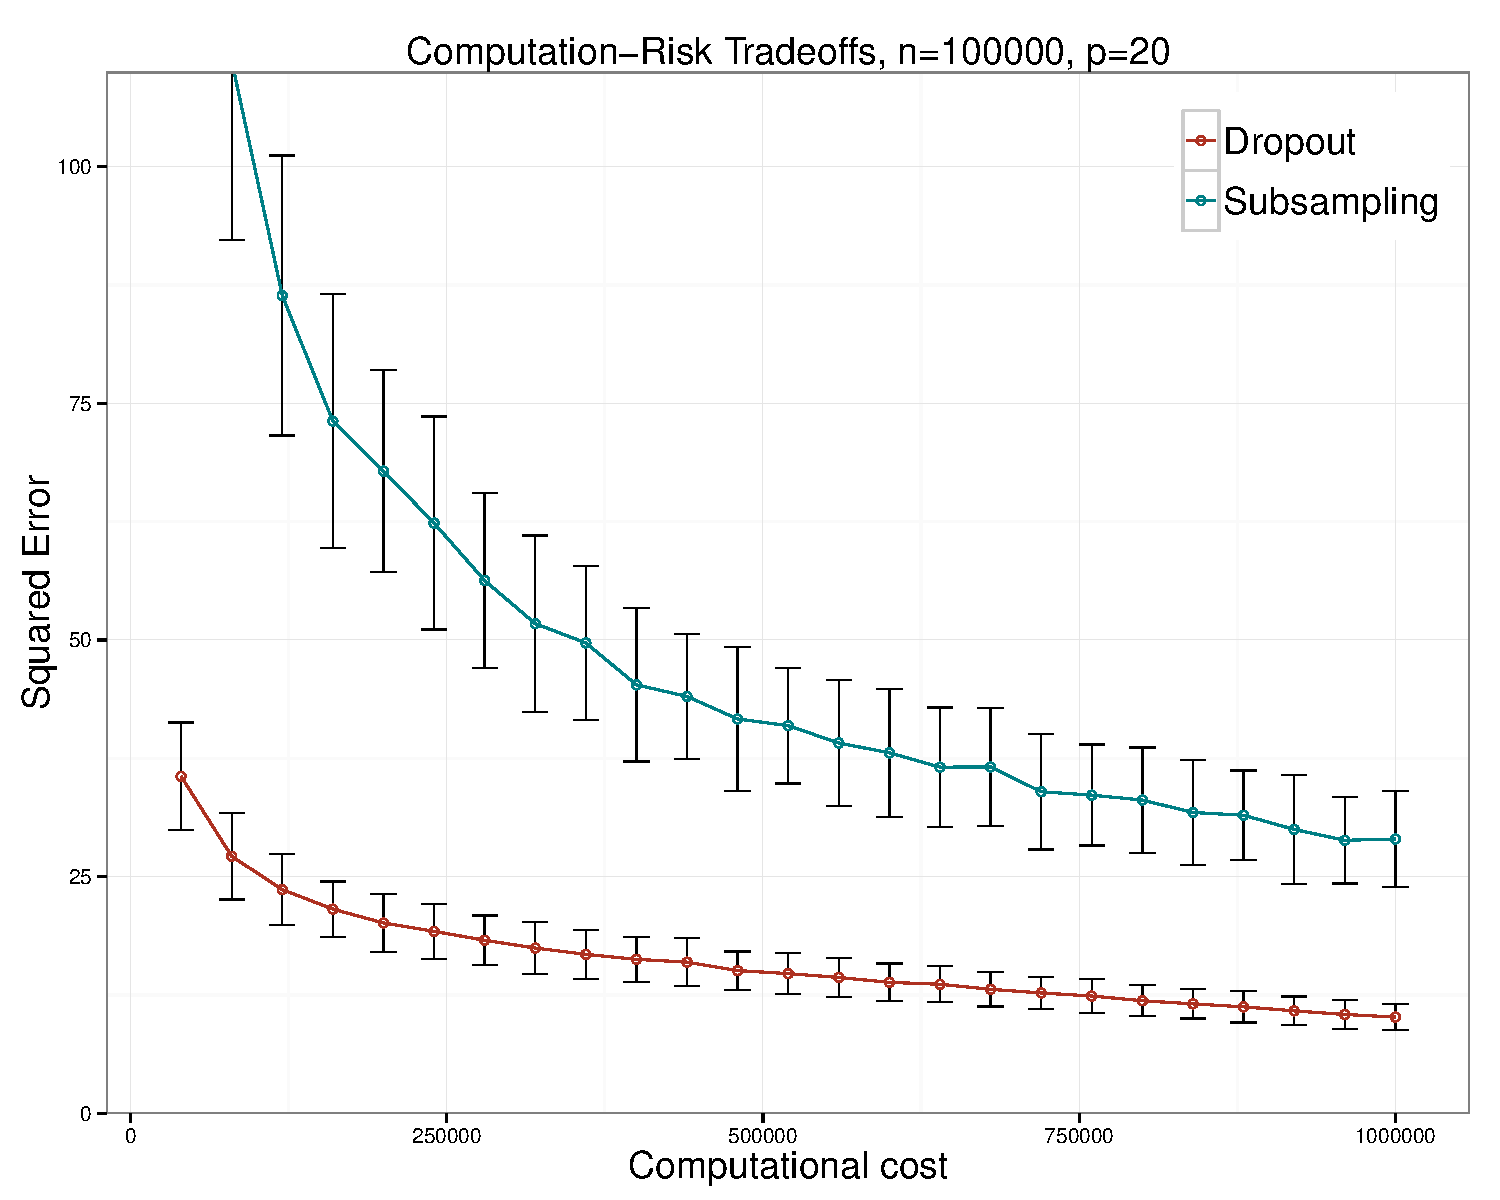
\includegraphics[width=.48\textwidth]{figs/dropout-subsample-n100000-p20-T100.pdf} &
\hskip-10pt
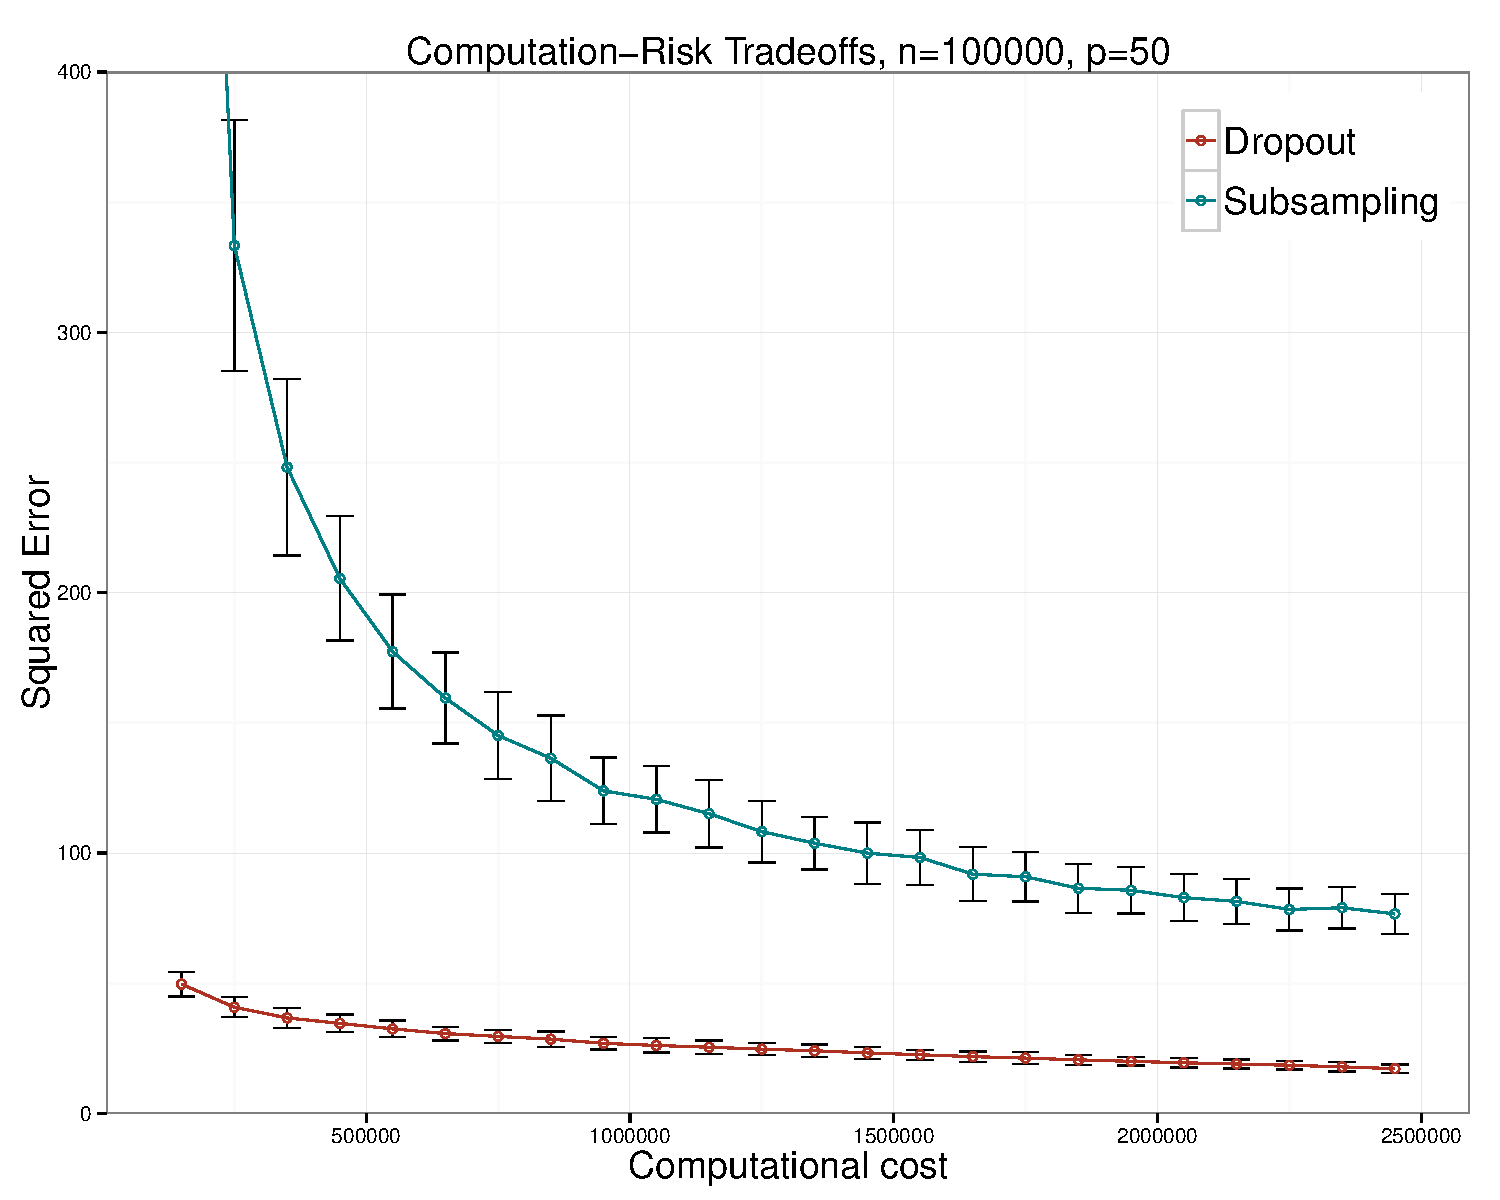
\includegraphics[width=.48\textwidth]{figs/dropout-subsample-n100000-p50-T100.pdf}
\end{tabular}
\end{center}
\caption{Comparision of subsampling to the dropout method for making
  computation-risk tradeoffs.  Two simulations are run, for $p=10$ and
  $p=20$ variables.  Subsampling with different subsample sizes $m$ is
  compared to the dropout with different dropout rates $\theta$.  The
  computational costs are measured by the theoretical bounds $O(mp^2 +
  p^3)$ for subsampling and $O(n\|\theta\|_1 + p^3)$ for the dropout,
  solved with subspace embedding. As $p$ increases, so does the
  relative advantage of the dropout.}
\label{fig:doss}
\end{figure}





